% Declaracao
\begin{center}
	Declaração de Autoria e de Direitos
\end{center}

\vspace{0.5cm}

Eu, \emph{\myName} CPF \emph{\myCpf}, autor da monografia \emph{\documentTitle}, subscrevo para os devidos fins, as seguintes informações:\\
1. O autor declara que o trabalho apresentado na disciplina de Projeto de Graduação da Escola Politécnica da UFRJ é de sua autoria, sendo original em forma e conteúdo.\\
2. Excetuam-se do item 1. eventuais transcrições de texto, figuras, tabelas, conceitos e idéias, que identifiquem claramente a fonte original, explicitando as autorizações obtidas dos respectivos proprietários, quando necessárias.\\
3. O autor permite que a UFRJ, por um prazo indeterminado, efetue em qualquer mídia de divulgação, a publicação do trabalho acadêmico em sua totalidade, ou em parte. Essa autorização não envolve ônus de qualquer natureza à UFRJ, ou aos seus representantes.\\
4. O autor pode, excepcionalmente, encaminhar à Comissão de Projeto de Graduação, a não divulgação do material, por um prazo máximo de 01 (um) ano, improrrogável, a contar da data de defesa, desde que o pedido seja justificado, e solicitado antecipadamente, por escrito, à Congregação da Escola Politécnica.\\
5. O autor declara, ainda, ter a capacidade jurídica para a prática do presente ato, assim como ter conhecimento do teor da presente Declaração, estando ciente das sanções e punições legais, no que tange a cópia parcial, ou total, de obra intelectual, o que se configura como violação do direito autoral previsto no Código Penal Brasileiro no art.184 e art.299, bem como na Lei 9.610.\\
6. O autor é o único responsável pelo conteúdo apresentado nos trabalhos acadêmicos publicados, não cabendo à UFRJ, aos seus representantes,  ou ao(s) orientador(es), qualquer responsabilização/ indenização nesse sentido.\\
7. Por ser verdade, firmo a presente declaração.\\

\vspace{0.5cm}
\begin{flushright}
    \parbox{10cm}{
        \centering
        \vspace{-1cm} % Ajuste o espaço entre a imagem e a linha
        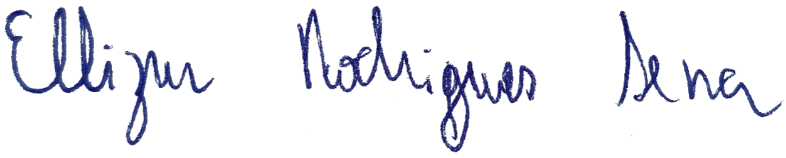
\includegraphics[height=1cm]{assinatura.png} \\ % Substitua "assinatura.png" pelo caminho da sua imagem
        \vspace{-0.8cm} % Ajuste o espaço entre a imagem e a linha
        \hrulefill

        \vspace{-0.375cm} % Ajuste o espaço entre a linha e o texto
        \centering{\myName}
		\vspace{0.1cm}
		}
\end{flushright}

\pagebreak

% Copyright
\vspace{0.5cm}

UNIVERSIDADE FEDERAL DO RIO DE JANEIRO \\
Escola Politécnica - Departamento de Eletrônica e de Computação \\
Centro de Tecnologia, bloco H, sala H-217, Cidade Universitária \\
Rio de Janeiro - RJ      CEP 21949-900\\
\vspace{0.5cm}
\paragraph{}Este exemplar é de propriedade da Universidade Federal do Rio de Janeiro, que poderá incluí-lo em base de dados, armazenar em computador, microfilmar ou adotar qualquer forma de arquivamento.
\paragraph{}É permitida a menção, reprodução parcial ou integral e a transmissão entre bibliotecas deste trabalho, sem modificação de seu texto, em qualquer meio que esteja ou venha a ser fixado, para pesquisa acadêmica, comentários e citações, desde que sem finalidade comercial e que seja feita a referência bibliográfica completa.
\paragraph{}Os conceitos expressos neste trabalho são de responsabilidade do(s) autor(es).


\pagebreak

% Dedicatória
%\begin{center}
%\textbf{DEDICATÓRIA}
%\end{center}
%      \vspace{0.5cm}

%\paragraph{}Opcional.

%\pagebreak


% Agradecimento
\begin{center}
	\textbf{AGRADECIMENTO}
\end{center}
\vspace{0.5cm}

\paragraph{}Agradeço à Deus, em primeiro lugar, porque acredito que sem ele nada é possível.

\paragraph{}Aos meus pais Helena Dias e Euzimar Sena, pelos conselhos e apoio em todos os momentos da minha vida.

\paragraph{}À minha esposa, Mayara Sena, pela companhia nas idas pro Fundão, por todo o incentivo e por todo apoio no desenvolvimento do trabalho.

\paragraph{}Aos meus amigos da UFRJ, Caroline Coelho, Pedro Lídio, João Pedro, Iuri Veloso e Breno Galves, por permanecerem comigo nos momentos bons e ruins.

\paragraph{}Aos meus supervisores da EPE, Kriseida Alekseev e Dan Gandelman, por me proporcionarem a primeira experiência profissional e por todo o incentivo a seguir carreira acadêmica.

\paragraph{}Ao meu orientador, José de Seixas, por aceitar me orientar e proporcionar a realização desse trabalho.

\paragraph{}Aos professores que gentilmente aceitaram fazer parte da minha banca, Natanael Júnior, José Gabriel e Kriseida Alekseev.

\pagebreak


% Resumo
\begin{center}
	\textbf{RESUMO}
\end{center}
\vspace{0.5cm}

\paragraph{} O biodiesel é um biocombustível renovável produzido de fontes vegetais e animais, desempenha um papel importante na transição energética global. A previsão precisa de seu preço é essencial para otimizar sua produção e comercialização, além de apoiar decisões no mercado de biocombustíveis, como o percentual obrigatório de mistura ao diesel.

\paragraph{} Este trabalho explora a aplicação de Redes Neurais Artificiais (\acsp{RNA}) e modelos estatísticos para prever o preço do biodiesel, aliados a modelos de extração de características, como tendência, ciclos senoidais e sazonais, para melhorar o desempenho das previsões. A pesquisa investiga o uso de diferentes modelos para prever o preço do biodiesel, considerando variáveis como o preço do óleo de soja e os preços de biodiesel por regiões do Brasil. As \acsp{RNA} foram escolhidas pela sua capacidade de modelar padrões não lineares e relações complexas entre essas variáveis.

\paragraph{} Os resultados mostram que as \acsp{RNA} têm bom desempenho na previsão do preço do biodiesel, obtendo medidas de desempenho melhores que os modelos estatísticos. Modelos menos profundos, como \acf{N-Linear} e \acf{MLP}, apresentaram melhor resultado nas previsões em comparação aos mais profundos, sugerindo que abordagens mais simples podem ser mais eficazes para capturar os padrões dinâmicos dos preços do biodiesel. Modelos morfológicos, com \acf{IMP} e \acf{IDLN}, também foram testados, mas não apresentaram desempenho satisfatório nas previsões.
\paragraph{}
\noindent Palavras-Chave: previsão de séries temporais, biodiesel, redes neurais, inteligência artificial, biocombustíveis, sustentabilidade.

\pagebreak


% Abstract
\begin{center}
	\textbf{ABSTRACT}
\end{center}
\vspace{0.5cm}

\paragraph{} Biodiesel is a renewable biofuel produced from plant and animal sources and plays an important role in the global energy transition. Accurately predicting its price is essential to optimize its production and commercialization, in addition to supporting decisions in the biofuel market, such as the mandatory percentage of blending with diesel.

\paragraph{} This work explores the application of Artificial Neural Networks (ANN) and statistical models to predict the price of biodiesel, combined with feature extraction models, such as trends, sinusoidal and seasonal cycles, to improve the performance of the predictions. The research investigates the use of different models to predict the price of biodiesel, considering variables such as the price of soybean oil and biodiesel prices by region of Brazil. ANN were chosen for their ability to model non-linear patterns and complex relationships between these variables.

\paragraph{} The results show that ANNs perform well in predicting biodiesel prices, obtaining better performance measures than statistical models. Shallower models, such as Normalized Linear (\acs{N-Linear}) and Multilayer Perceptron (\acs{MLP}), performed better in predictions compared to deeper ones, suggesting that simpler approaches may be more effective in capturing the dynamic patterns of biodiesel prices.Morphological models, with Increasing-Decreasing Linear Neuron (\acs{IDLN}) and Increasing Morphological Perceptron (\acs{IMP}), were also tested, but did not show satisfactory performance in the predictions.
\paragraph{}
\noindent Key-words: time series forecasting, biodiesel, neural networks, artificial intelligence, biofuels, sustainability.

\pagebreak


% Siglas
\begin{center}
	\textbf{LISTA DE ABREVIATURAS}
\end{center}
\vspace{0.5cm}

%\input{acronyms}
\printacronyms[heading=none]


\pagebreak







